\chapter{Stack e Code}

\section{Introduzione}

Stack e code sono strutture dati lineari astratte che impongono regole specifiche sull'ordine di accesso agli elementi. A differenza di array e liste, dove possiamo accedere a qualsiasi posizione, stack e code permettono accesso solo agli estremi della sequenza.

Queste restrizioni, lungi dall'essere limitazioni, rendono stack e code strumenti potentissimi per modellare situazioni reali e risolvere problemi algoritmici fondamentali.

\section{Stack (Pila)}

\subsection{Definizione e proprietà}

\begin{definizione}[Stack]
Uno \textbf{stack} (o pila) è una struttura dati lineare che segue il principio \textbf{LIFO} (Last In, First Out): l'ultimo elemento inserito è il primo ad essere rimosso.
\end{definizione}

\textbf{Metafora:} Una pila di piatti. Puoi aggiungere un piatto in cima, e puoi rimuovere solo il piatto in cima.

\textbf{Operazioni fondamentali:}
\begin{itemize}
    \item \texttt{push(x)}: Inserisce l'elemento $x$ in cima allo stack
    \item \texttt{pop()}: Rimuove e restituisce l'elemento in cima
    \item \texttt{top()}/\texttt{peek()}: Restituisce l'elemento in cima senza rimuoverlo
    \item \texttt{isEmpty()}: Verifica se lo stack è vuoto
    \item \texttt{size()}: Restituisce il numero di elementi
\end{itemize}

\textbf{Visualizzazione:}

\begin{center}
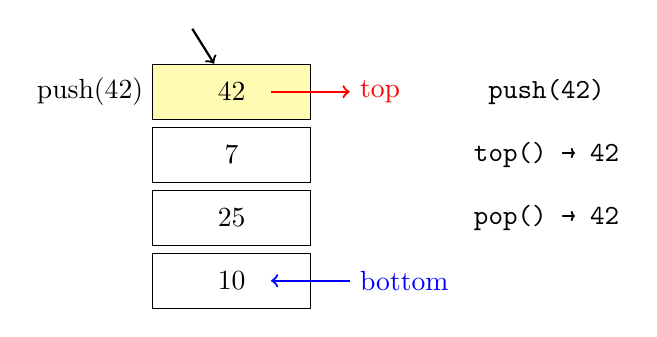
\begin{tikzpicture}[
    box/.style={rectangle, draw, minimum width=2cm, minimum height=0.7cm}
]
    \node[box] (b1) at (0,0) {10};
    \node[box] (b2) at (0,0.8) {25};
    \node[box] (b3) at (0,1.6) {7};
    \node[box, fill=yellow!30] (b4) at (0,2.4) {42};

    \draw[->, thick, red] (0.5, 2.4) -- (1.5, 2.4) node[right] {top};

    \node[left] at (-1, 2.4) {push(42)};
    \draw[->, thick] (-0.5, 3.2) -- (b4);

    \draw[<-, thick, blue] (0.5, 0) -- (1.5, 0) node[right] {bottom};

    % Rappresentazione delle operazioni
    \node at (4, 2.4) {\texttt{push(42)}};
    \node at (4, 1.6) {\texttt{top() → 42}};
    \node at (4, 0.8) {\texttt{pop() → 42}};
\end{tikzpicture}
\end{center}

\subsection{Implementazione con array}

\begin{lstlisting}[style=pseudocode]
class StackArray:
    def __init__(self, capacità):
        self.array = nuovo array di dimensione capacità
        self.top = -1  // indice dell'elemento in cima
        self.capacità = capacità

    def isEmpty(self):
        return self.top == -1

    def isFull(self):
        return self.top == self.capacità - 1

    def push(self, x):
        """
        Inserisce x in cima
        Complessità: O(1)
        """
        if self.isFull():
            errore "Stack overflow"

        self.top = self.top + 1
        self.array[self.top] = x

    def pop(self):
        """
        Rimuove e restituisce l'elemento in cima
        Complessità: O(1)
        """
        if self.isEmpty():
            errore "Stack underflow"

        x = self.array[self.top]
        self.top = self.top - 1
        return x

    def peek(self):
        """
        Restituisce l'elemento in cima senza rimuoverlo
        Complessità: O(1)
        """
        if self.isEmpty():
            errore "Stack vuoto"

        return self.array[self.top]

    def size(self):
        return self.top + 1
\end{lstlisting}

\textbf{Analisi:}
\begin{itemize}
    \item Tutte le operazioni sono $O(1)$
    \item Spazio: $O(n)$ dove $n$ è la capacità
    \item Svantaggio: capacità fissa
\end{itemize}

\subsection{Implementazione con lista concatenata}

\begin{lstlisting}[style=pseudocode]
class StackLista:
    def __init__(self):
        self.top = None
        self.dimensione = 0

    def isEmpty(self):
        return self.top == None

    def push(self, x):
        """
        Inserisce x in cima
        Complessità: O(1)
        """
        nuovo = Nodo(x)
        nuovo.next = self.top
        self.top = nuovo
        self.dimensione = self.dimensione + 1

    def pop(self):
        """
        Rimuove e restituisce l'elemento in cima
        Complessità: O(1)
        """
        if self.isEmpty():
            errore "Stack underflow"

        x = self.top.dato
        self.top = self.top.next
        self.dimensione = self.dimensione - 1
        return x

    def peek(self):
        if self.isEmpty():
            errore "Stack vuoto"
        return self.top.dato

    def size(self):
        return self.dimensione
\end{lstlisting}

\textbf{Vantaggi:}
\begin{itemize}
    \item Nessuna capacità massima
    \item Tutte le operazioni sono $O(1)$
\end{itemize}

\textbf{Svantaggi:}
\begin{itemize}
    \item Overhead dei puntatori
    \item Peggiore località di cache
\end{itemize}

\subsection{Applicazioni degli stack}

\subsubsection{Valutazione di espressioni}

Gli stack sono fondamentali per valutare espressioni aritmetiche.

\textbf{Esempio: Espressioni postfisse (notazione polacca inversa)}

Nell'espressione postfissa, gli operatori seguono gli operandi:
\begin{itemize}
    \item Infissa: $(3 + 4) \times 5$
    \item Postfissa: $3\ 4\ +\ 5\ \times$
\end{itemize}

\begin{lstlisting}[style=pseudocode]
def ValutaPostfissa(espressione):
    """
    Valuta un'espressione postfissa
    Input: array di token (numeri e operatori)
    Output: risultato
    Complessità: O(n)
    """
    stack = Stack()

    for token in espressione:
        if token è un numero:
            stack.push(token)
        else:  // token è un operatore
            b = stack.pop()
            a = stack.pop()

            if token == '+':
                risultato = a + b
            elif token == '-':
                risultato = a - b
            elif token == '*':
                risultato = a * b
            elif token == '/':
                risultato = a / b

            stack.push(risultato)

    return stack.pop()
\end{lstlisting}

\textbf{Esempio di esecuzione:} Espressione $3\ 4\ +\ 5\ \times$

\begin{center}
\begin{tabular}{|c|c|l|}
\hline
\textbf{Token} & \textbf{Stack} & \textbf{Azione} \\
\hline
3 & [3] & push 3 \\
4 & [3, 4] & push 4 \\
+ & [7] & pop 4, pop 3, push 3+4 \\
5 & [7, 5] & push 5 \\
$\times$ & [35] & pop 5, pop 7, push 7×5 \\
\hline
\end{tabular}
\end{center}

Risultato: 35

\textbf{Conversione da infissa a postfissa (Shunting Yard Algorithm):}

\begin{lstlisting}[style=pseudocode]
def InfissaAPostfissa(espressione):
    """
    Converte espressione infissa in postfissa
    Algoritmo di Dijkstra (Shunting Yard)
    Complessità: O(n)
    """
    output = []
    stack = Stack()

    precedenza = {'+': 1, '-': 1, '*': 2, '/': 2}

    for token in espressione:
        if token è un numero:
            output.append(token)

        elif token == '(':
            stack.push(token)

        elif token == ')':
            while not stack.isEmpty() and stack.peek() != '(':
                output.append(stack.pop())
            stack.pop()  // rimuove '('

        elif token è un operatore:
            while (not stack.isEmpty() and
                   stack.peek() != '(' and
                   precedenza[stack.peek()] >= precedenza[token]):
                output.append(stack.pop())
            stack.push(token)

    while not stack.isEmpty():
        output.append(stack.pop())

    return output
\end{lstlisting}

\subsubsection{Bilanciamento di parentesi}

Problema: Verificare se le parentesi in un'espressione sono bilanciate.

\begin{lstlisting}[style=pseudocode]
def ParentesiBilanciate(espressione):
    """
    Verifica bilanciamento parentesi/bracket/braces
    Input: stringa con caratteri (), [], {}
    Output: True se bilanciate, False altrimenti
    Complessità: O(n)
    """
    stack = Stack()
    aperture = {'(', '[', '{'}
    chiusure = {')', ']', '}'}
    match = {'(': ')', '[': ']', '{': '}'}

    for char in espressione:
        if char in aperture:
            stack.push(char)

        elif char in chiusure:
            if stack.isEmpty():
                return False

            top = stack.pop()
            if match[top] != char:
                return False

    return stack.isEmpty()
\end{lstlisting}

\textbf{Esempi:}
\begin{itemize}
    \item \texttt{"((()))"} → True
    \item \texttt{"([)"]"} → False (ordine sbagliato)
    \item \texttt{"((("} → False (non chiuse)
\end{itemize}

\subsubsection{Backtracking e ricorsione}

Lo stack di sistema (call stack) gestisce le chiamate ricorsive. Ogni chiamata di funzione aggiunge un \textit{frame} allo stack contenente variabili locali e indirizzo di ritorno.

\textbf{Esempio: Fattoriale}

\begin{lstlisting}[style=pseudocode]
def Fattoriale(n):
    if n == 0:
        return 1
    else:
        return n * Fattoriale(n-1)
\end{lstlisting}

Per \texttt{Fattoriale(3)}, lo stack evolve così:

\begin{center}
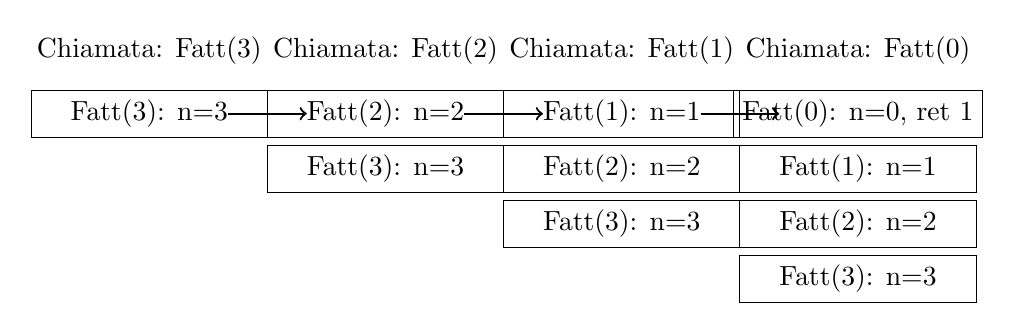
\begin{tikzpicture}[
    frame/.style={rectangle, draw, minimum width=3cm, minimum height=0.6cm}
]
    % Passo 1
    \node at (0, 3) {Chiamata: Fatt(3)};
    \node[frame] at (0, 2.2) {Fatt(3): n=3};

    % Passo 2
    \node at (3, 3) {Chiamata: Fatt(2)};
    \node[frame] at (3, 2.2) {Fatt(2): n=2};
    \node[frame] at (3, 1.5) {Fatt(3): n=3};

    % Passo 3
    \node at (6, 3) {Chiamata: Fatt(1)};
    \node[frame] at (6, 2.2) {Fatt(1): n=1};
    \node[frame] at (6, 1.5) {Fatt(2): n=2};
    \node[frame] at (6, 0.8) {Fatt(3): n=3};

    % Passo 4
    \node at (9, 3) {Chiamata: Fatt(0)};
    \node[frame] at (9, 2.2) {Fatt(0): n=0, ret 1};
    \node[frame] at (9, 1.5) {Fatt(1): n=1};
    \node[frame] at (9, 0.8) {Fatt(2): n=2};
    \node[frame] at (9, 0.1) {Fatt(3): n=3};

    \draw[->, thick] (1, 2.2) -- (2, 2.2);
    \draw[->, thick] (4, 2.2) -- (5, 2.2);
    \draw[->, thick] (7, 2.2) -- (8, 2.2);
\end{tikzpicture}
\end{center}

Poi lo stack si svuota man mano che le funzioni ritornano: $1 \to 1 \to 2 \to 6$.

\subsubsection{Percorsi in profondità (DFS)}

Il Depth-First Search usa uno stack (esplicito o tramite ricorsione) per esplorare grafi.

\subsubsection{Undo/Redo}

Editor di testo e software di grafica usano due stack: uno per undo, uno per redo.

\begin{lstlisting}[style=pseudocode]
class Editor:
    def __init__(self):
        self.undo_stack = Stack()
        self.redo_stack = Stack()

    def eseguiAzione(self, azione):
        azione.esegui()
        self.undo_stack.push(azione)
        self.redo_stack.clear()  // invalida redo

    def undo(self):
        if not self.undo_stack.isEmpty():
            azione = self.undo_stack.pop()
            azione.annulla()
            self.redo_stack.push(azione)

    def redo(self):
        if not self.redo_stack.isEmpty():
            azione = self.redo_stack.pop()
            azione.esegui()
            self.undo_stack.push(azione)
\end{lstlisting}

\section{Code (Queue)}

\subsection{Definizione e proprietà}

\begin{definizione}[Coda]
Una \textbf{coda} (queue) è una struttura dati lineare che segue il principio \textbf{FIFO} (First In, First Out): il primo elemento inserito è il primo ad essere rimosso.
\end{definizione}

\textbf{Metafora:} Una coda di persone in fila. Chi arriva prima viene servito prima.

\textbf{Operazioni fondamentali:}
\begin{itemize}
    \item \texttt{enqueue(x)}: Inserisce l'elemento $x$ in coda
    \item \texttt{dequeue()}: Rimuove e restituisce l'elemento in testa
    \item \texttt{front()}: Restituisce l'elemento in testa senza rimuoverlo
    \item \texttt{isEmpty()}: Verifica se la coda è vuota
    \item \texttt{size()}: Restituisce il numero di elementi
\end{itemize}

\textbf{Visualizzazione:}

\begin{center}
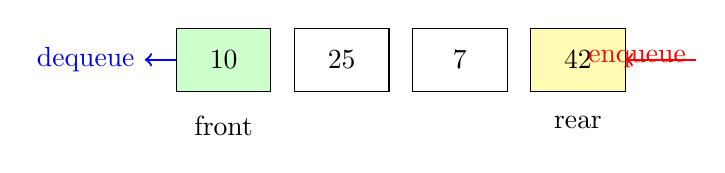
\begin{tikzpicture}[
    box/.style={rectangle, draw, minimum width=1.2cm, minimum height=0.8cm}
]
    \node[box, fill=green!20] (b1) at (0,0) {10};
    \node[box] (b2) at (1.5,0) {25};
    \node[box] (b3) at (3,0) {7};
    \node[box, fill=yellow!30] (b4) at (4.5,0) {42};

    \draw[->, thick, blue] (b1) -- (-1, 0) node[left] {dequeue};
    \draw[->, thick, red] (6, 0) -- (b4) node[right] {enqueue};

    \node[below] at (0, -0.6) {front};
    \node[below] at (4.5, -0.6) {rear};
\end{tikzpicture}
\end{center}

\subsection{Implementazione con array circolare}

Per evitare di sprecare spazio quando facciamo dequeue, usiamo un \textbf{array circolare}: quando raggiungiamo la fine dell'array, "avvolgiamo" all'inizio.

\begin{lstlisting}[style=pseudocode]
class QueueArray:
    def __init__(self, capacità):
        self.array = nuovo array di dimensione capacità
        self.front = 0
        self.rear = -1
        self.dimensione = 0
        self.capacità = capacità

    def isEmpty(self):
        return self.dimensione == 0

    def isFull(self):
        return self.dimensione == self.capacità

    def enqueue(self, x):
        """
        Inserisce x in coda
        Complessità: O(1)
        """
        if self.isFull():
            errore "Queue overflow"

        self.rear = (self.rear + 1) % self.capacità
        self.array[self.rear] = x
        self.dimensione = self.dimensione + 1

    def dequeue(self):
        """
        Rimuove e restituisce l'elemento in testa
        Complessità: O(1)
        """
        if self.isEmpty():
            errore "Queue underflow"

        x = self.array[self.front]
        self.front = (self.front + 1) % self.capacità
        self.dimensione = self.dimensione - 1
        return x

    def getFront(self):
        if self.isEmpty():
            errore "Queue vuota"
        return self.array[self.front]

    def size(self):
        return self.dimensione
\end{lstlisting}

\textbf{Visualizzazione array circolare:}

\begin{center}
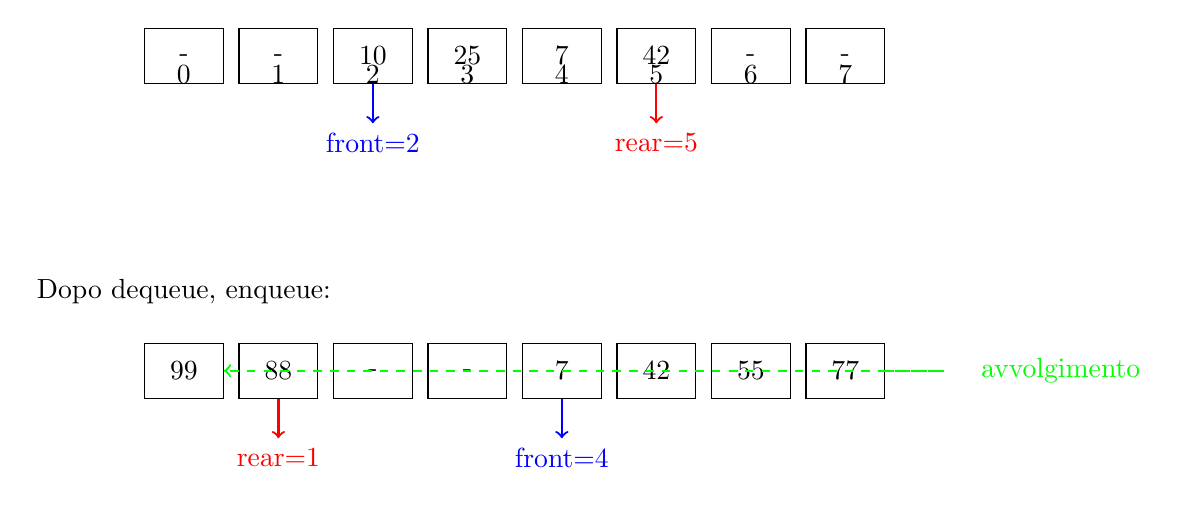
\begin{tikzpicture}[
    box/.style={rectangle, draw, minimum width=1cm, minimum height=0.7cm}
]
    \foreach \i in {0,...,7} {
        \node[box] (a\i) at (\i*1.2, 0) {};
    }

    \node at (a0) {-};
    \node at (a1) {-};
    \node at (a2) {10};
    \node at (a3) {25};
    \node at (a4) {7};
    \node at (a5) {42};
    \node at (a6) {-};
    \node at (a7) {-};

    \draw[->, thick, blue] (a2.south) -- ++(0, -0.5) node[below] {front=2};
    \draw[->, thick, red] (a5.south) -- ++(0, -0.5) node[below] {rear=5};

    \node[below] at (a0) {0};
    \node[below] at (a1) {1};
    \node[below] at (a2) {2};
    \node[below] at (a3) {3};
    \node[below] at (a4) {4};
    \node[below] at (a5) {5};
    \node[below] at (a6) {6};
    \node[below] at (a7) {7};

    % Dopo alcuni dequeue e enqueue, avvolgimento
    \node at (0, -3) {Dopo dequeue, enqueue:};
    \foreach \i in {0,...,7} {
        \node[box] (b\i) at (\i*1.2, -4) {};
    }

    \node at (b0) {99};
    \node at (b1) {88};
    \node at (b2) {-};
    \node at (b3) {-};
    \node at (b4) {7};
    \node at (b5) {42};
    \node at (b6) {55};
    \node at (b7) {77};

    \draw[->, thick, blue] (b4.south) -- ++(0, -0.5) node[below] {front=4};
    \draw[->, thick, red] (b1.south) -- ++(0, -0.5) node[below] {rear=1};

    \draw[->, thick, green, dashed] (b7.east) to[out=0, in=0] (b0.east);
    \node[right, green] at (10, -4) {avvolgimento};
\end{tikzpicture}
\end{center}

\subsection{Implementazione con lista concatenata}

\begin{lstlisting}[style=pseudocode]
class QueueLista:
    def __init__(self):
        self.front = None
        self.rear = None
        self.dimensione = 0

    def isEmpty(self):
        return self.front == None

    def enqueue(self, x):
        """
        Inserisce x in coda
        Complessità: O(1)
        """
        nuovo = Nodo(x)

        if self.isEmpty():
            self.front = nuovo
            self.rear = nuovo
        else:
            self.rear.next = nuovo
            self.rear = nuovo

        self.dimensione = self.dimensione + 1

    def dequeue(self):
        """
        Rimuove e restituisce l'elemento in testa
        Complessità: O(1)
        """
        if self.isEmpty():
            errore "Queue underflow"

        x = self.front.dato
        self.front = self.front.next

        if self.front == None:  // coda ora vuota
            self.rear = None

        self.dimensione = self.dimensione - 1
        return x

    def getFront(self):
        if self.isEmpty():
            errore "Queue vuota"
        return self.front.dato

    def size(self):
        return self.dimensione
\end{lstlisting}

\subsection{Applicazioni delle code}

\subsubsection{Sistemi operativi}

\textbf{Scheduling dei processi:} I processi pronti per l'esecuzione sono mantenuti in una coda. Lo scheduler seleziona il primo processo (FIFO).

\textbf{Buffer di stampa:} I documenti da stampare sono accodati e stampati nell'ordine di arrivo.

\subsubsection{Breadth-First Search (BFS)}

L'algoritmo BFS per grafi usa una coda per esplorare i nodi livello per livello.

\begin{lstlisting}[style=pseudocode]
def BFS(grafo, sorgente):
    """
    Visita in ampiezza di un grafo
    Complessità: O(V + E)
    """
    visitato = insieme vuoto
    coda = Queue()

    coda.enqueue(sorgente)
    visitato.add(sorgente)

    while not coda.isEmpty():
        u = coda.dequeue()
        print(u)  // processa u

        for v in grafo.adiacenti(u):
            if v not in visitato:
                visitato.add(v)
                coda.enqueue(v)
\end{lstlisting}

\subsubsection{Gestione delle richieste}

\textbf{Server web:} Le richieste HTTP sono accodate e processate in ordine FIFO.

\textbf{Call center:} Le chiamate sono accodate e gli operatori rispondono nell'ordine di arrivo.

\subsection{Code con priorità (Priority Queue)}

\begin{definizione}[Coda con priorità]
Una \textbf{coda con priorità} è una struttura dati in cui ogni elemento ha una priorità associata. L'elemento con priorità più alta viene rimosso per primo.
\end{definizione}

\textbf{Operazioni:}
\begin{itemize}
    \item \texttt{insert(x, priorità)}: Inserisce $x$ con la priorità data
    \item \texttt{extractMax()}: Rimuove e restituisce l'elemento con priorità massima
    \item \texttt{getMax()}: Restituisce (senza rimuovere) l'elemento con priorità massima
\end{itemize}

Le code con priorità sono tipicamente implementate con \textbf{heap} (capitolo successivo).

\textbf{Applicazioni:}
\begin{itemize}
    \item Algoritmo di Dijkstra (cammini minimi)
    \item Algoritmo di Prim (minimum spanning tree)
    \item Scheduling con priorità
    \item Simulazione di eventi discreti
\end{itemize}

\subsection{Deque (Double-Ended Queue)}

\begin{definizione}[Deque]
Una \textbf{deque} (pronuncia "deck") è una coda doppia: si possono inserire e rimuovere elementi da entrambe le estremità.
\end{definizione}

\textbf{Operazioni:}
\begin{itemize}
    \item \texttt{insertFront(x)}, \texttt{insertRear(x)}
    \item \texttt{deleteFront()}, \texttt{deleteRear()}
    \item \texttt{getFront()}, \texttt{getRear()}
\end{itemize}

\textbf{Implementazione efficiente:} Lista doppiamente concatenata o array circolare.

\textbf{Proprietà interessante:} Una deque può simulare sia uno stack che una coda!

\section{Confronto delle strutture}

\begin{center}
\begin{tabular}{|l|c|c|}
\hline
\textbf{Operazione} & \textbf{Stack} & \textbf{Queue} \\
\hline
Inserimento & $O(1)$ (push) & $O(1)$ (enqueue) \\
Rimozione & $O(1)$ (pop) & $O(1)$ (dequeue) \\
Accesso in cima/testa & $O(1)$ & $O(1)$ \\
Accesso arbitrario & $O(n)$ & $O(n)$ \\
Ricerca & $O(n)$ & $O(n)$ \\
Spazio & $O(n)$ & $O(n)$ \\
\hline
\textbf{Principio} & LIFO & FIFO \\
\hline
\end{tabular}
\end{center}

\section{Teoremi e proprietà}

\begin{teorema}[Complessità delle operazioni]
In uno stack o coda implementati correttamente (con array o lista), tutte le operazioni fondamentali (push/pop/enqueue/dequeue) hanno complessità $\Theta(1)$ nel caso peggiore.
\end{teorema}

\begin{teorema}[Simulazione]
\begin{enumerate}
    \item Due stack possono simulare una coda (con operazioni ammortizzate $O(1)$)
    \item Una coda NON può simulare efficacemente uno stack
    \item Una deque può simulare sia stack che code con tutte le operazioni $O(1)$
\end{enumerate}
\end{teorema}

\begin{proof}[Dimostrazione del punto 1]
Usiamo due stack: \texttt{inbox} e \texttt{outbox}.

\textbf{Enqueue:} Push su \texttt{inbox} -- $O(1)$

\textbf{Dequeue:}
\begin{itemize}
    \item Se \texttt{outbox} non è vuoto: pop da \texttt{outbox} -- $O(1)$
    \item Altrimenti: sposta tutti gli elementi da \texttt{inbox} a \texttt{outbox} (invertendone l'ordine), poi pop da \texttt{outbox}
\end{itemize}

Il costo ammortizzato è $O(1)$ perché ogni elemento viene spostato al più una volta.
\end{proof}

\section{Esercizi}

\subsection{Esercizio 1}
Implementare una funzione che inverte uno stack usando un solo stack ausiliario.

\subsection{Esercizio 2}
Implementare uno stack che supporta anche l'operazione \texttt{getMin()} in $O(1)$.

\subsection{Esercizio 3}
Data una sequenza di operazioni push/pop, verificare se produce un output valido. Es: push(1), push(2), pop(), push(3), pop(), pop() → [2, 3, 1] è valido?

\subsection{Esercizio 4}
Implementare una coda usando due stack e dimostrare che il costo ammortizzato di dequeue è $O(1)$.

\subsection{Esercizio 5}
Scrivere un algoritmo che, data un'espressione infissa, la valuti direttamente usando due stack (uno per operandi, uno per operatori).

\section{Conclusioni}

Stack e code sono strutture dati fondamentali che, nonostante la loro semplicità concettuale, hanno applicazioni vastissime:

\begin{itemize}
    \item \textbf{Stack}: Ricorsione, backtracking, parsing, valutazione espressioni, undo/redo
    \item \textbf{Code}: Scheduling, BFS, gestione eventi, buffer, simulazioni
\end{itemize}

\textbf{Punti chiave:}
\begin{itemize}
    \item Stack = LIFO, Code = FIFO
    \item Tutte le operazioni sono $O(1)$
    \item Implementabili con array o liste
    \item Array circolari per code efficienti
    \item Code con priorità richiedono heap
    \item Deque generalizza stack e code
\end{itemize}

La scelta tra implementazione con array o lista dipende da:
\begin{itemize}
    \item Array: migliore località di cache, dimensione massima nota
    \item Lista: dimensione dinamica illimitata, ma overhead di puntatori
\end{itemize}

Queste strutture sono i building block per algoritmi più complessi che vedremo nei prossimi capitoli.
